% !TEX root = ../diary-book.tex

\section{令和6年12月29日 シャワー測定頻度の推定（続き）}
\subsection{ミュオンの一次宇宙線依存性}

2024-12-29 13:54:53

12月21日に引き続きシミュレーションのまとめを行っている。
1~GeV から 100~TeV までの一次宇宙線が 20~km 上空から入射してきたときの、ミュオンの平均観測数とシャワーの観測効率についてのまとめを行う。

12月21日の計算では、10~MeV以上のエネルギーを持つ任意の粒子が3個以上のサイトで観測された場合について効率を求めており、ミューオンも 100~m 四方の領域で観測された場合についての個数をカウントしている。

効率についての条件は粒子の種類、エネルギーについて再検討すべきであり、ミューオンの個数についてもどのように面積平均を取っていくかは良く検討する必要がある。

ひとまず手のひら毎秒1個のミューオンについての一次宇宙線の寄与度について調べたいところ。

角度積分で毎秒1個一次宇宙線が到来する面積で、生成されたミューオンの粒子すを平均すれば、毎秒あたりのミューオン生成数の寄与度に変換できる気がする。数学的に正しいかどうかはまだ確認していない。

毎秒１個一次宇宙線が到来する面積に対応する円内に存在するミュオンの平均数をその面積で割ればよい。

宇宙線のフラックス $F$ (m$^{2}\cdot$sr$\cdot$s$\cdot$GeV)$^{-1}$ は E~(GeV) に対して以下のように表すことができる

\begin{equation}
   F = 10^{4.7143} E^{-3.045}
\end{equation}

立体角 $\pi$/4 (現時点でこれは適当)くらいの粒子が使えるとして、1~TeV の宇宙線は 1~TeV程度の広がりを持っていると仮定して、それぞれのエネルギーでの到来頻度に直すにはエネルギーをかければ良い。

\begin{equation}
   F = \pi/4 * 10^{4.7} E^{-2.045}
\end{equation}

が 1~m$^2$ あたり毎秒あたりの到来頻度となる。したがって１秒に１個到来する面積はこれの逆数を取ればよい。

\begin{figure}
   \centering
   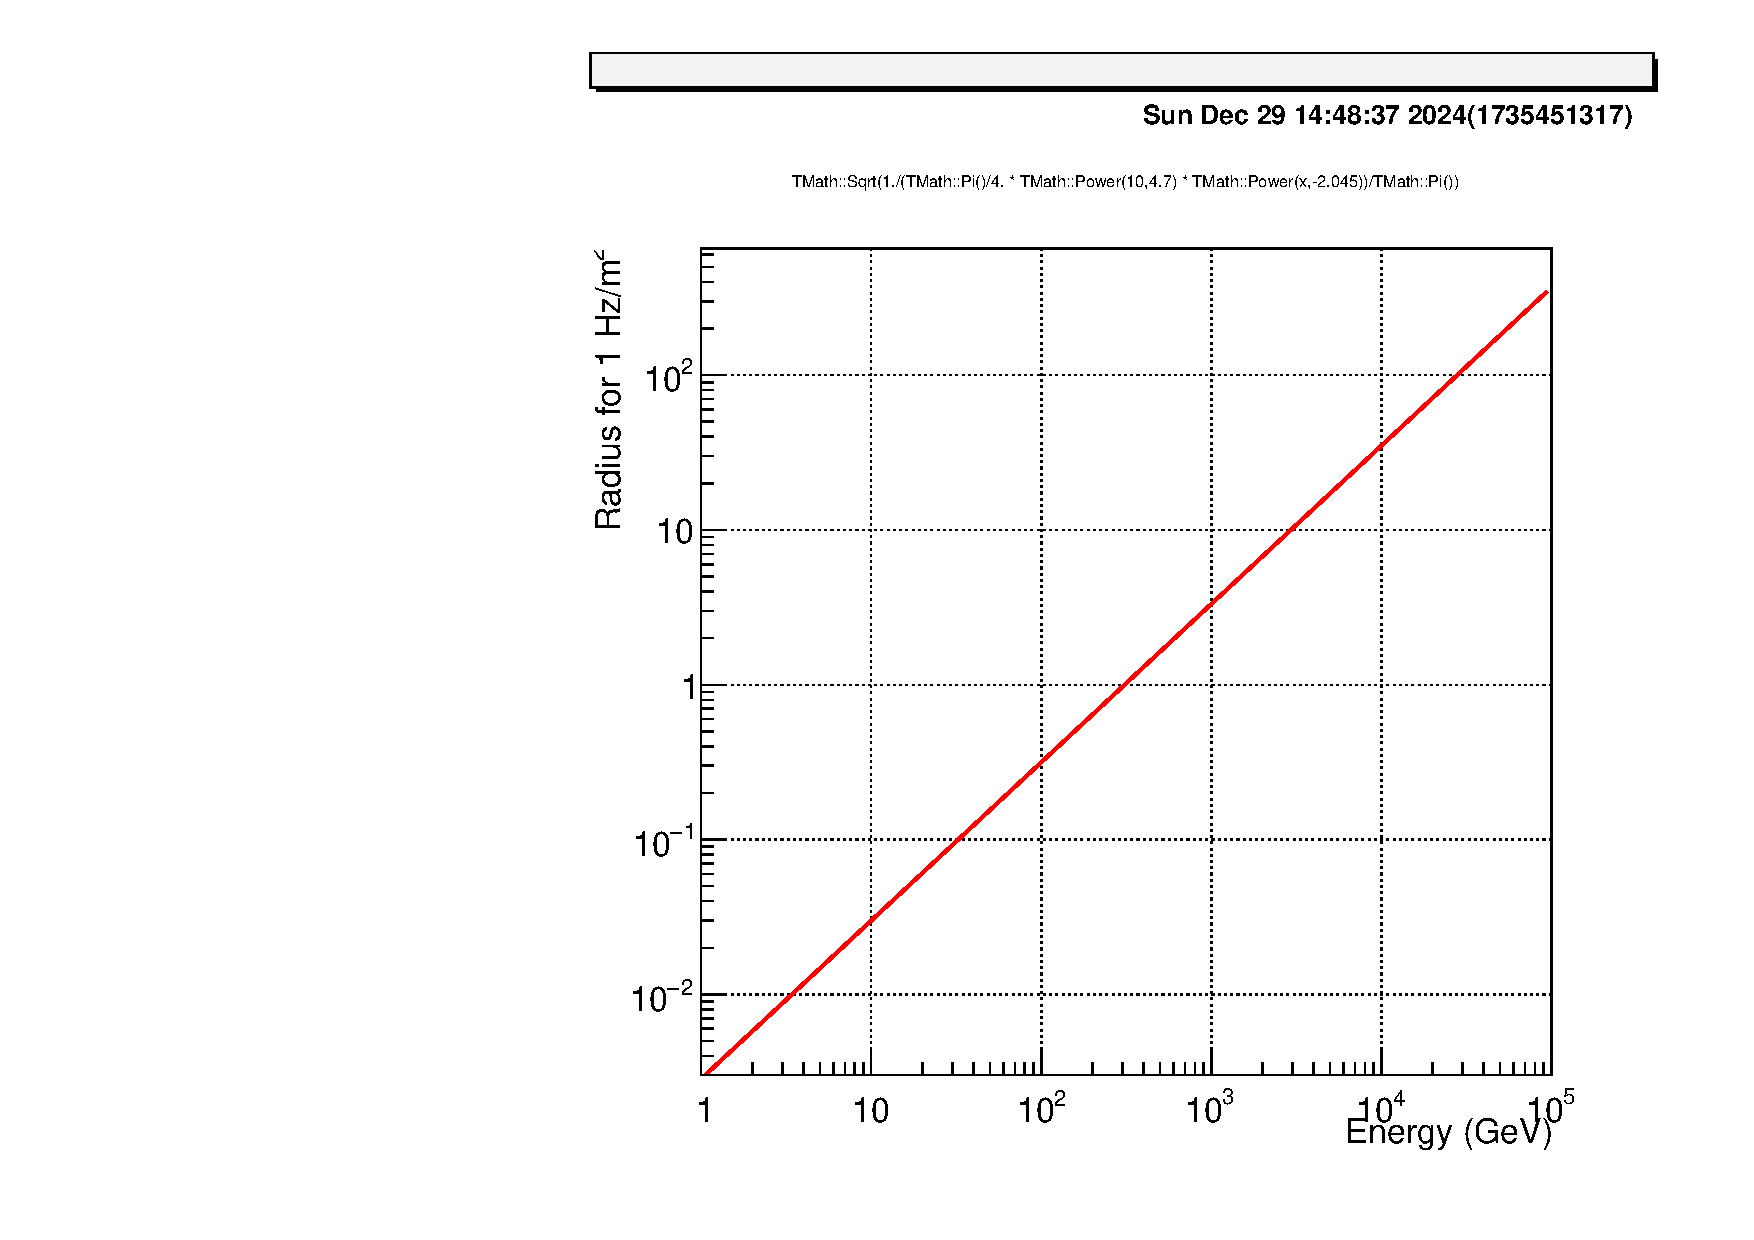
\includegraphics[width=.7\linewidth]{../../figs/ata03/figs/20241229/1735451317.pdf}
   \label{1平方メートルあたり毎秒あたり1個の宇宙線を観測するために必要な円の半径を示したもの}
\end{figure}

エネルギーによってミュオンの広がりが異なるので、半径分布になおして、その半値全幅をとって基準の面積とすることにする。この面積内の平均数と宇宙線到来数を掛け算したものが当該エネルギーでの分布ということにする。

\begin{figure}
   \begin{center}
      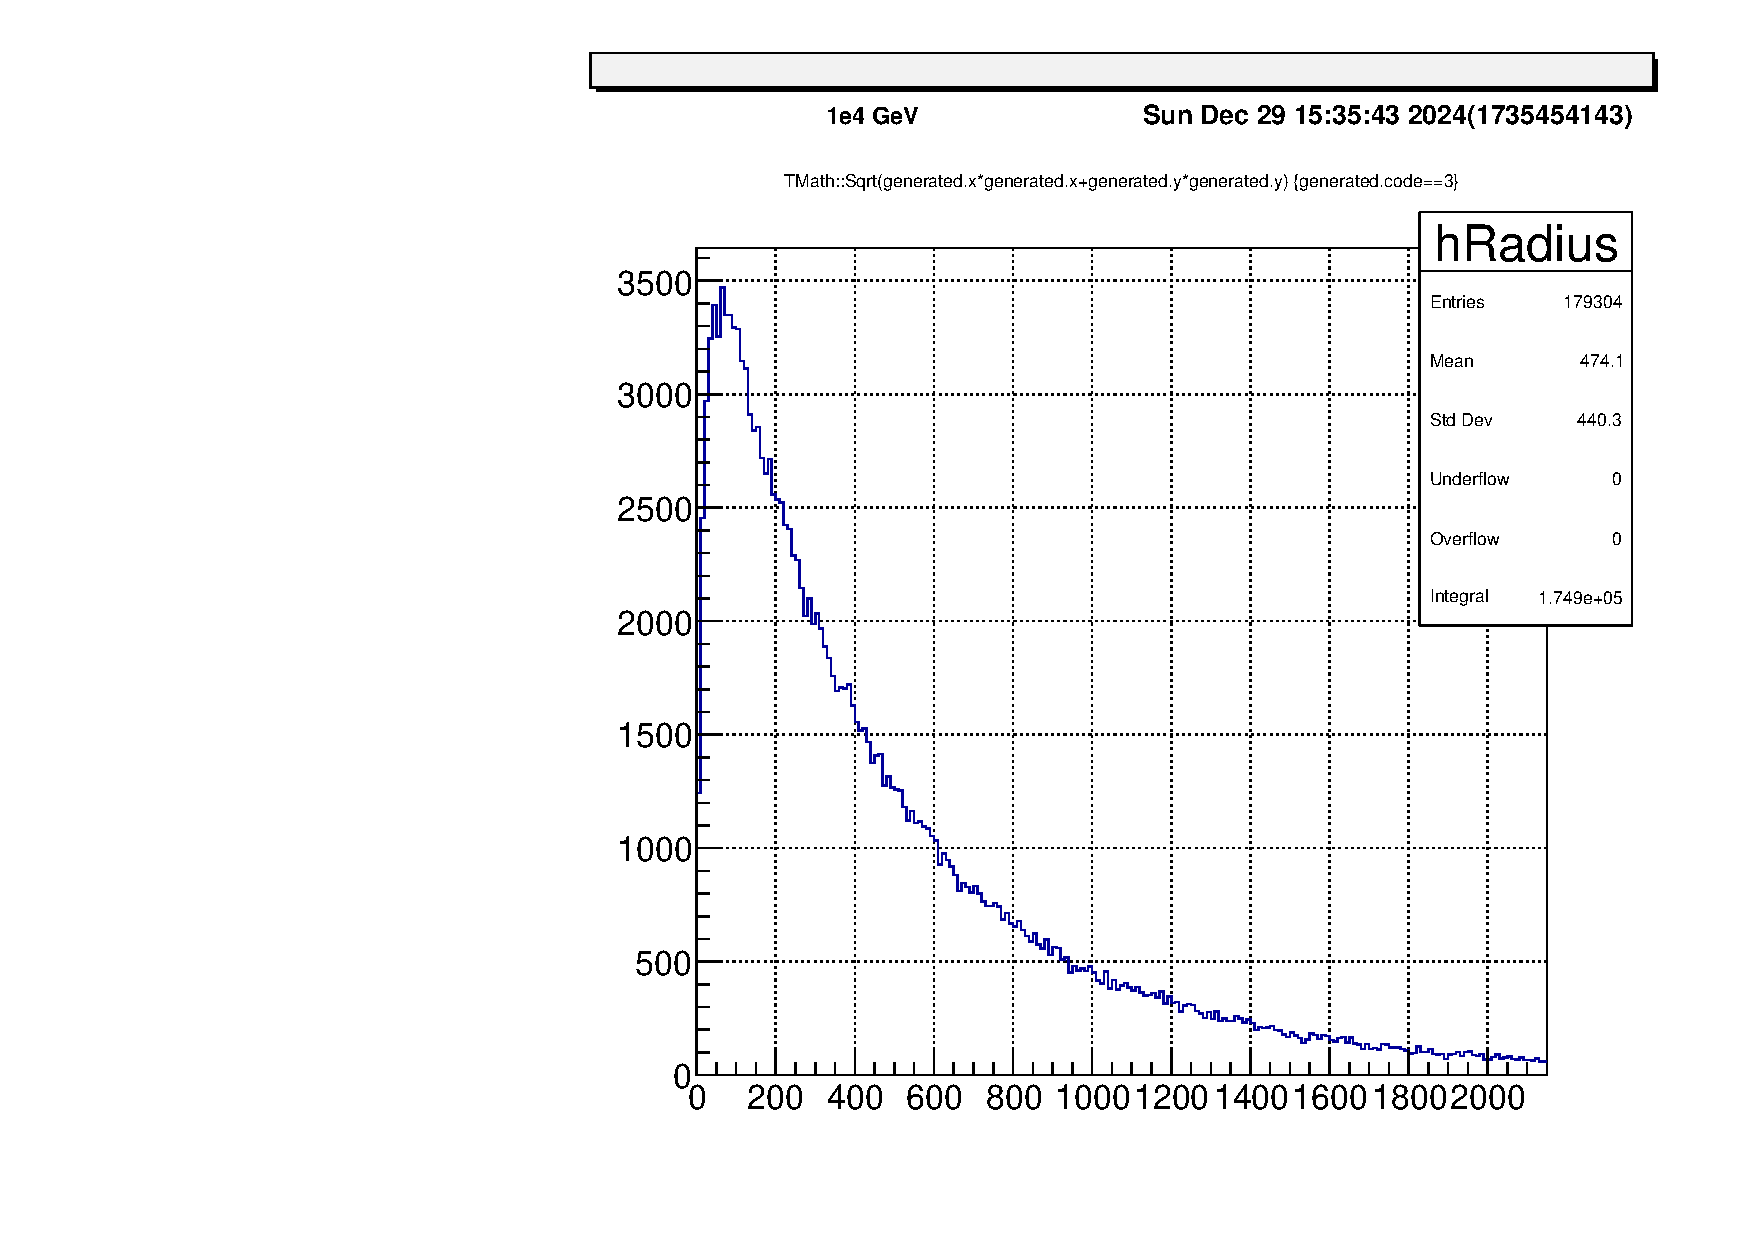
\includegraphics[width=.7\linewidth]{../../figs/ata03/figs/20241229/1735454143.pdf}
   \end{center}
   \label{10 $^4$ GeVのときの半径分布。これの半値の距離をつかって面積を導出する。}
\end{figure}

（以下はおそらく誤りというか焦点が異なる。）
上の例では、10$^{4}$~GeVの宇宙線に対するミュオンの生成分布を表示している。積分は 350~m 程度までおこなって 92710e-3 個のミュオンが生成されているので 0.24e-3~個/m$^{2}$のミュオン数となる。半径 350~m 離れたところの宇宙線まで寄与することができると考える。10$^{4}$~GeV の宇宙線の到来数は 0.00025994 個/秒/m$^{2}$ なので、350~m の領域には 100.0個/sの宇宙線が到来している。したがって 24e-3~個/m$^{2}$/s のミュオンが 10$^{4}$~GeVの宇宙線から生成されているという計算になる。

2024-12-29 16:30:16

上記の考え方はシャワー面法に有効なミュオンの個数を考える際には重要な概念といえる。コア付近でのみシャワーの再構成が可能となるため、有効活用できるミュオンの数は減るためである。一方で今やりたいと思っている、手のひら毎秒1個のミュオンに対する一次宇宙線の寄与度については全ミュオンの数を積分してよいので、単純に1シャワーあたりの個数と一次宇宙線の頻度をかければ良いということになる。

(以上、2024-12-29 16:32:46)

